\documentclass[a4paper, 12pt, titlepage]{article}

\usepackage{graphicx, color} %for å inkludere grafikk
\usepackage{verbatim, color} %for å inkludere filer med tegn LaTeX ikke liker. \verbatiminput{verb.txt}
%\usepackage{gensymb} %gensymb Symbols Defined to Work in Both Math and Text Mode 

\usepackage[T1]{fontenc} %for å bruke æøå. upgrades to 256 bit encoding. More characters
\usepackage[utf8]{inputenc} %Kan forandres til latin1. utf8 gir norske tegn
%inputenc allows the user to input accented characters directly from the keyboard;
%fontenc is oriented to output, that is, what fonts to use for printing characters.
%\usepackage[norsk]{babel} 

\usepackage{pdfpages} %Importing external pdf-pages
\usepackage[compact]{titlesec} %Spacing for two-column document

\usepackage{textcomp} % make degrees centigrade symbols, euros, etc
\usepackage{amsmath, amssymb} %e.g. \begin{theorem}[Pythagoras], \begin{proof} or {align}
\usepackage{amsbsy, amsfonts} %\pmb for annerledes boldfont
\usepackage{parskip} %Space between paragraphs
\usepackage{float} %Im­proves the in­ter­face for defin­ing float­ing ob­jects such as fig­ures and ta­bles.
\usepackage{simplewick}
\usepackage{libertine} 
\usepackage{siunitx} % SI units. Example: \SI{100}{\micro\meter}

\usepackage{geometry} % Definerer marger. 
 %\geometry{headhight=1mm}
 \geometry{top=20mm, bottom=20mm, left=34mm, right=34mm} % Marger i mm. Total bredde er 210mm



\author{Wilhelm Holmen}
\title{FYS4411 Project 1}

\begin{document}
 \maketitle
 \newpage

 \section*{1a}
 In this exercise I will use Monte Carlo integration to compute the expectation value for the energy. 
 \begin{align*}
 	\left< E \right> = \frac{\int d \mathbf{r_1} d \mathbf{r_2} \psi_T^*(r_1,r_2) \hat H \psi_T(r_1,r_2)}{\int d \mathbf{r_1} d \mathbf{r_2} \psi_T^*(r_1,r_2) \psi_T(r_1,r_2)}
 \end{align*}
 I need a wavefunction for this, so first I choose the ground state wavefunction solution the hydrogen atom, $e^{-\alpha r}$, for both the particles. This gives the total wavefunction
 \begin{align*}
 	\Psi_T(r_1,r_2) = e^{-\alpha(r_1 + r_2)}
 \end{align*}
 This is not the correct wavefunction, but it can give a decent first evaluation. 

 In the Metropolis algorithm, I will check wether a move given by, $\mathbf{R^{'}} = \mathbf{R} + \delta \cdot r $, will be accepted. $r$ is a random number in $[0,1]$. The acceptance criteria is given by
 \begin{align*}
 	\frac{P(\mathbf{R^{'}} )}{P(\mathbf{R} )} = \frac{\int d \mathbf{R^{'}} \psi^*_T(\mathbf{R^{'}} ) \psi_T(\mathbf{R^{'}} )}{\int d \mathbf{R} \psi^*_T(\mathbf{R}) \psi_T(\mathbf{R} )} \geq r
 \end{align*}

 Because of the variational princible, the trial energy will always be higher than the true energy. Therefore we can adjust $\alpha$ and the steplength $\delta$ until we get the lowest possible energy. The best steplength $\delta$ is a steplength that will accept around $50\%$ of the proposed steps. Using an algorithm that loops over different steplengths, I adjust $\alpha$ and plot the energy and variance as a function of $\alpha$. I start the steplength at $\delta = 1.2$ and increase it by $0.5*r$, $r \in [0,1]$ for each step. Testing if the number of accepted steps are within $[0.49,0.51]$ I either accept the step length or increase it.  

 \begin{figure}[H]
 	\centering
 	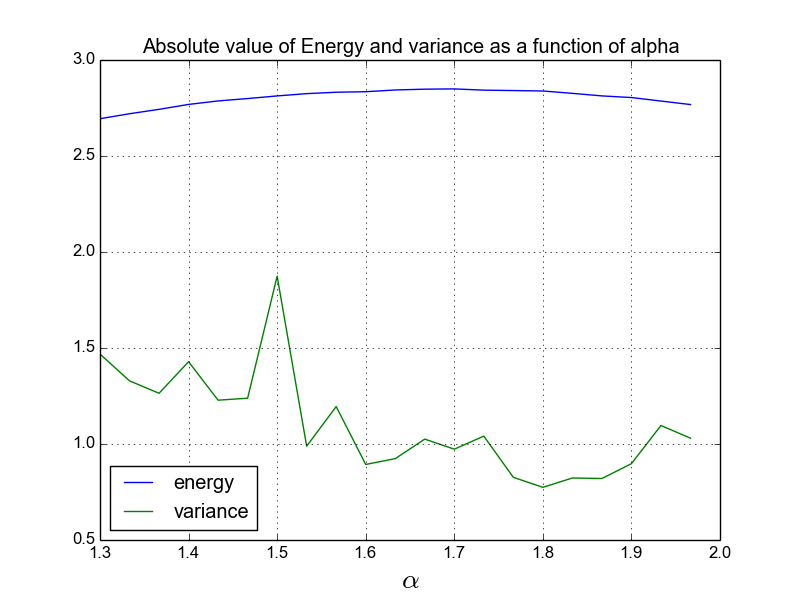
\includegraphics[width=\textwidth]{../python_programs/EnergyVariance_helium1.png}
 \end{figure}

 By looking closer at the energy and variance around $\alpha = 1.68$, we see that we get an energy of $\left<E\right> = -2.84997$, with a variance of $\sigma ^2 = 0.932912$. This is pretty close to the real value of $E_{exact} = -2.903$. We see however that the variance is smaller for $\alpha = 1.8$, $1.9$ and $1.6$.
 
 \begin{figure}[H]
 	\centering
 	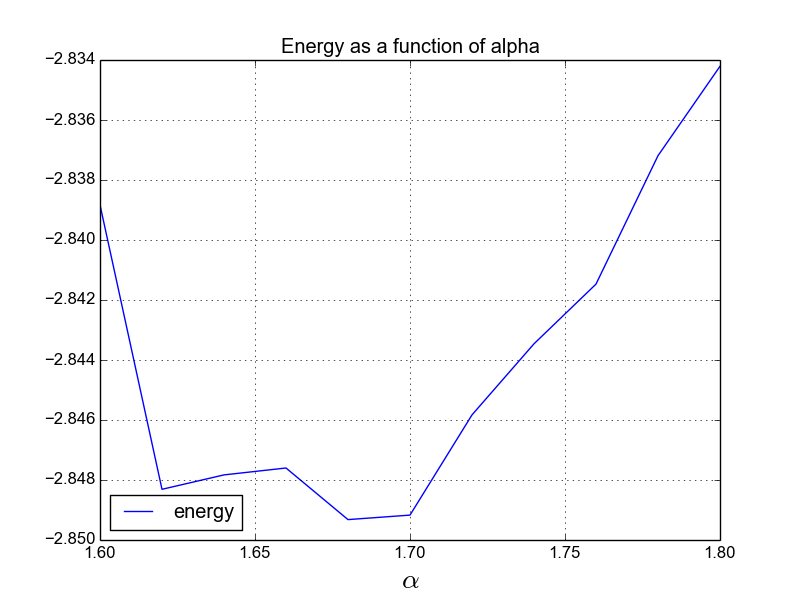
\includegraphics[width=\textwidth]{../python_programs/EnergyVariance_helium2.png}
 \end{figure}

 \begin{figure}[H]
 	\centering
 	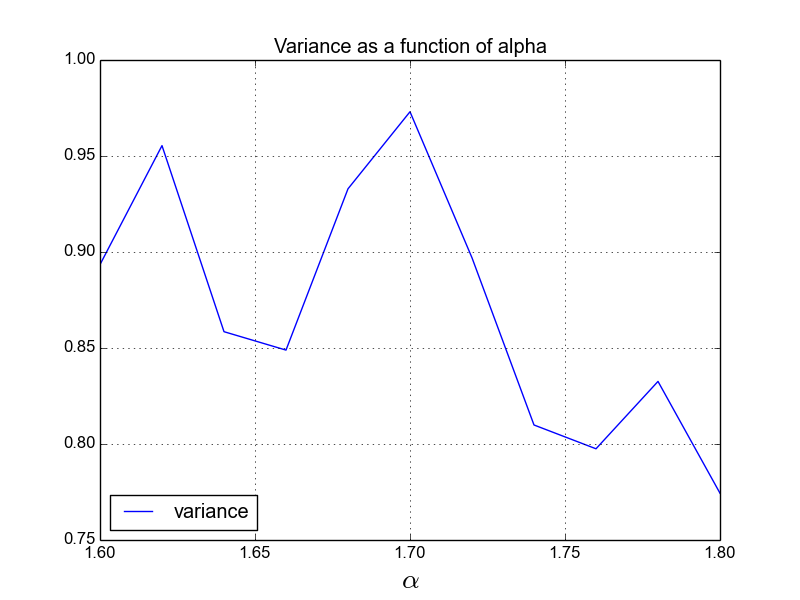
\includegraphics[width=\textwidth]{../python_programs/EnergyVariance_helium3.png}
 \end{figure}

 We can get a better result by improving our test function, $\Psi_T$. We can introduce a Jastrow factor. Here $r_{12} = |r_1 - r_2|$. 
 \begin{align*}
 	\Psi_T(r_1,r_2) = e^{-\alpha(r_1 + r_2)}e^{\frac{r_{12}}{2(1+\beta r_{12})}}
 \end{align*}
 
 Setting $\beta = 1.0$, we see that we can achieve a better energy, namely $\left<E\right> = -2.88013$. 
 \begin{figure}[H]
 	\centering
 	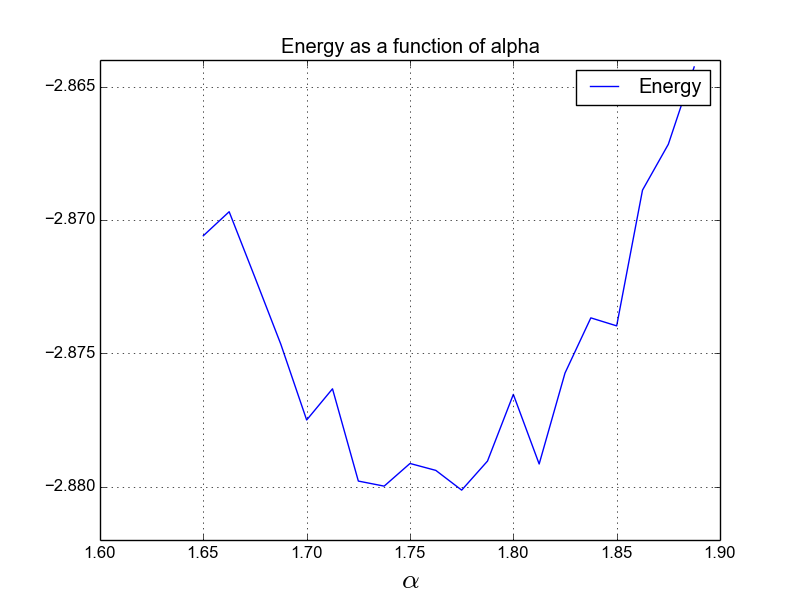
\includegraphics[width=\textwidth]{../python_programs/EnergyVariance_helium4.png}
 \end{figure}
 \begin{figure}[H]
 	\centering
 	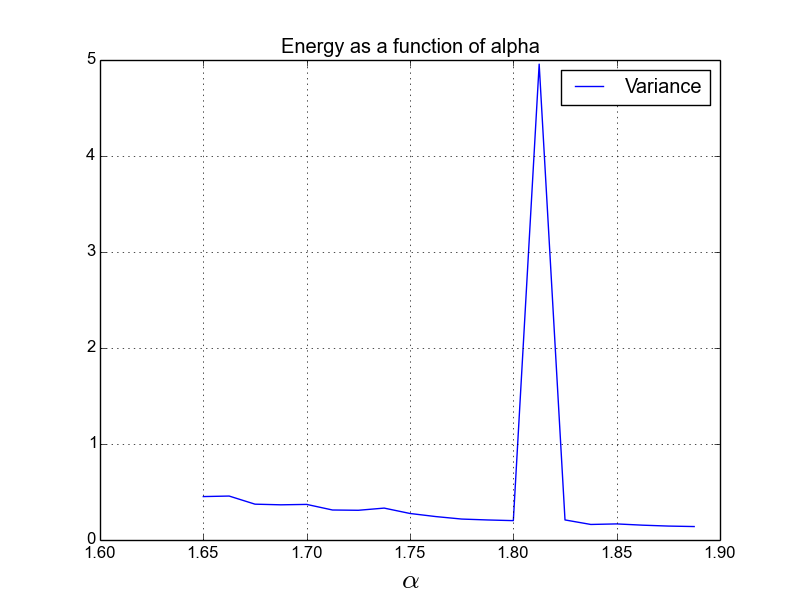
\includegraphics[width=\textwidth]{../python_programs/EnergyVariance_helium5.png}
 \end{figure}

\section*{b}
\begin{align*}
	\Psi_T &= e^{-\alpha(r_1 + r_2)} \\
	E_L &= \frac{1}{\Psi_T} \hat H \Psi_T \\
	\hat H &= -\frac{1}{2}\nabla_1^2 - \frac{1}{2}\nabla_2^2 - \frac{2}{r_1} - \frac{2}{r_2} + \frac{1}{r_{12}} \\
	\nabla_1^2 \Psi_T &= \frac{1}{r_1^2}\frac{\partial}{\partial r_1}\left(r_1^2 \frac{\partial \Psi_T}{\partial r_1}\right) = -\frac{2}{r_1}\alpha \Psi_T + \alpha^2\Psi_T
\end{align*}
Combining these calculations, we get the expression for the local energy. 
\begin{align*}
	E_L &= (\alpha - 2) \left( \frac{1}{r_1} + \frac{1}{r_2}\right) + \frac{1}{r_{12}} - \alpha^2
\end{align*}
Now finding the closed-form expression for $E_L$ for the second wavefunction. 
\begin{align*}
	\Psi_T = e^{-\alpha(r_1 + r_2)}e^{\frac{r_{12}}{2(1+\beta r_{12})}}
\end{align*}
First looking at
\begin{align*}
	\nabla_1^2 \Psi_T = \frac{1}{r_1^2}\frac{\partial}{\partial r_1}\left(r_1^2 \frac{\partial \Psi_T}{\partial r_1}\right)
\end{align*}
\begin{align*}
	\frac{\partial \Psi_T}{\partial r_1}
\end{align*}

A quick Sympy program computes the following expressions for the local energy:
\begin{align*}
- 1.0 \alpha^{2} + \frac{1.0 \alpha}{r_{2}} + \frac{1.0 \alpha}{r_{1}} - \frac{2}{r_{2}} + \frac{1}{r_{12}} - \frac{2}{r_{1}}\end{align*}


\section*{Importance Sampling}
 Introducing importance sampling. We can see from the plot below that using $dt = 10^-3$, we get stable results. A smaller $dt$ probably gives rise to different kinds of errors, like truncation errors etc. Using this dt, we get $-2.86462$ as the energy. This is a slightly higher energy than the energy obtained in 
 \begin{figure}[H] 
 	\centering
 	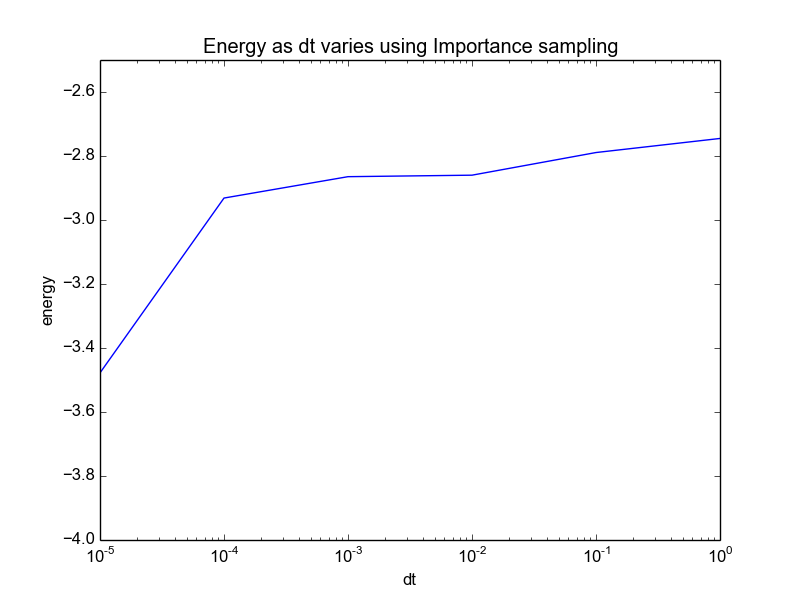
\includegraphics[width=\textwidth]{../python_programs/ImportanceSampling_Helium_dt.png}
 \end{figure}

\section*{Statistical Analysis}
 A Monte Carlo simulation gives rise to two kinds of error. Systematic errors and statistical errors. Systematic errors are due to limitations of the applied models and faulty implementations. Here I will explore methods to estimate the statistical error. 

 Given a set of local energies, the variance is a measure of the spread from the true mean. The definition is
 \begin{align*}
 	\text{Var}(E) = \left< E^2 \right> - \left< E \right> ^2 
 \end{align*}
 Unfortunatly we do not know the true mean in a Monte-Carlo simulation. The computed average $\overline E$ is an approximation to the exact mean, and we do the following approximation
 \begin{align*}
 	\text{Var}(E) \approx \overline{E^2} - \overline{E}^2 
 \end{align*}
 For the case where we have the exact wave function, the variance becomes $0$, so the variance is an excellent measure of how close we are to the exact wave function. The variance however is \textit{not} a direct measure of the error. The standard deviation, the square root of the variance is related of the \textit{spread} in the sampled value. 
 \begin{align}
 	\sigma ^2(x) = \text{Var}(x)
 	\label{deviation}
 \end{align}
 This does not account for the samples being corrolated. Two samples, $x$ and $y$ are corrolated if the \textit{Covariance} is non-zero.
 \begin{align*}
 	\text{Cov}(x,y) = \left< xy \right> - \left< x \right> \left<y \right> 
 \end{align*}
 The diagonal elements of the Covariance is the Variance. By ignoring the corrolations, one get an error estimate that is generally too small. Given the true deviation, $\sigma_e$ and $\sigma$ from \ref{deviation} we have
 \begin{align*}
 	\sigma_c \geq \sigma
 \end{align*}

 The most interesting quantity when doing statistical analysis is not the error of single samples. It is the error of the mean value. One can show that the variance for the mean value, $m$ is 
 \begin{align*}
 	\sigma^2 (m) = \frac{1}{n} \text{Cov}(x) = \frac{1}{n^2} \sum_{k,l=1}^n (x_k - m)(x_l - m )
 \end{align*}
 Where n is the number of samples used to calculate $m$ and 
 \begin{align*}
 	m = \frac{1}{n} \sum_i^n x_i
 \end{align*}
 Calculating the Covariance is an expensive process for a large sample set, so we need a better way to calculate this. 

\section*{Blocking}
 There is no need to do statistical analysis within the Monte-Carlo simulation. By storing the data set, one can estimate the error post process. An efficient algorithm for this is called blocking. 

 Given a set of $N$ samples from a single Monte-Carlo process. This set is divided into $n$ blocks of size $n_b = N/n$. Now we can treat each block as an individual simulation to calculate the variance of a calculated mean, $m$. 
 \begin{align*}
 	\sigma^2 (m) = \left<m^2\right> - \left<m\right>^2 
 \end{align*}

\section*{One-body density}
 The one-body density is defined as
 \begin{align*}
 	\rho(r_1) = \int_{r_2} .. \int_{r_N} | \Phi(r_1 r_2 .. r_N) |^2 dr_2 .. dr_N
 \end{align*}

 The distribution $|\Phi(r)|^2$ describes the distribution of a particle in the system. The one-body density $\rho(r_1)$ describes the simultaneous distribution of every particle in the system. $\rho(r_1) dr_1 $ represents the probability of finding \textit{any} particle in the volume element $dr_1$ as oppsed to $|\Phi(r)|^2$ giving the probability of finding \textit{particle $r_1$} in the volume element $dr_1$. Due to the indistinguishable nature of the particles, any of the coordinates contain information about all the particles. I will therefore normalize this density to the number of particles $N$ and not $1$ which is common for the one-particle density. 

 The way this is computed in a Monte Carlo simulation is by taking snapshots of all positions for every timestep, then constructing a histogram to construct an approximation to the wave function.

 The charge density for a single particle is given by 
 \begin{align*}
 	\rho_q (r) = q |\Psi(r)|^2
 \end{align*}
 However, since we already have computed the many-body probability density, we can use this instead to get the many-body charge density of the system. 
 \begin{align*}
 	\rho_q (r) = Q \rho(r_1)
 \end{align*}

\section*{Variational Monte Carlo on Helium}
 I have found the optimal parametres for calculating on Helium. I set $\alpha = 1.68$ and $\beta = 0.3$. When doing a 

\end{document}


